\documentclass[10pt,letterpaper]{article}
\usepackage[margin=.82in]{geometry}
\usepackage[T1]{fontenc}\usepackage{lmodern,graphicx,booktabs,amsmath,xcolor,hyperref,xurl,caption,fancyhdr}
\hypersetup{colorlinks=true,urlcolor=teal,linkcolor=teal,pdftitle={Check a modeled retrofit choice against another weather case},pdfauthor={James Jean}}
\pagestyle{fancy}\fancyhf{}\fancyhead[L]{\small Retrofit weather choice / Study 27}\fancyhead[R]{\small Independent simulation case study}\fancyfoot[C]{\thepage}
\setlength{\headheight}{14pt}\setlength{\parindent}{0pt}\setlength{\parskip}{6pt}\captionsetup{font=small,labelfont=bf,hypcap=false}
\begin{document}
{\small\color{teal} RETROFIT SCREENING / DECISION SENSITIVITY\par}
\vspace{7pt}{\LARGE\bfseries Check a modeled retrofit choice against another weather case\par}
\vspace{6pt}James Jean \hfill 30 October 2026
\section*{The decision}
A building-energy model can help screen alternatives, but a first-place result deserves another question: does the choice persist under another supplied scenario? This study compares four separate retrofit measures and no action in two published ComStock weather-year simulation cases for one Vermont county. It evaluates simple decision rules without adding an unnecessary prediction model.

\textbf{Finding.} Among 112 held Hotel and Warehouse model cases, 17 have a different unique top-ranked measure across the two cases. Maximin changes the nominal 2018 choice in 8 cases; minimax regret changes it in 10. Mean worst-case regret is 0.119 percentage points for nominal and 0.053 for minimax regret. That last inequality follows from the stated optimization objective; it is \emph{not evidence of field savings or a new method}.

\begin{center}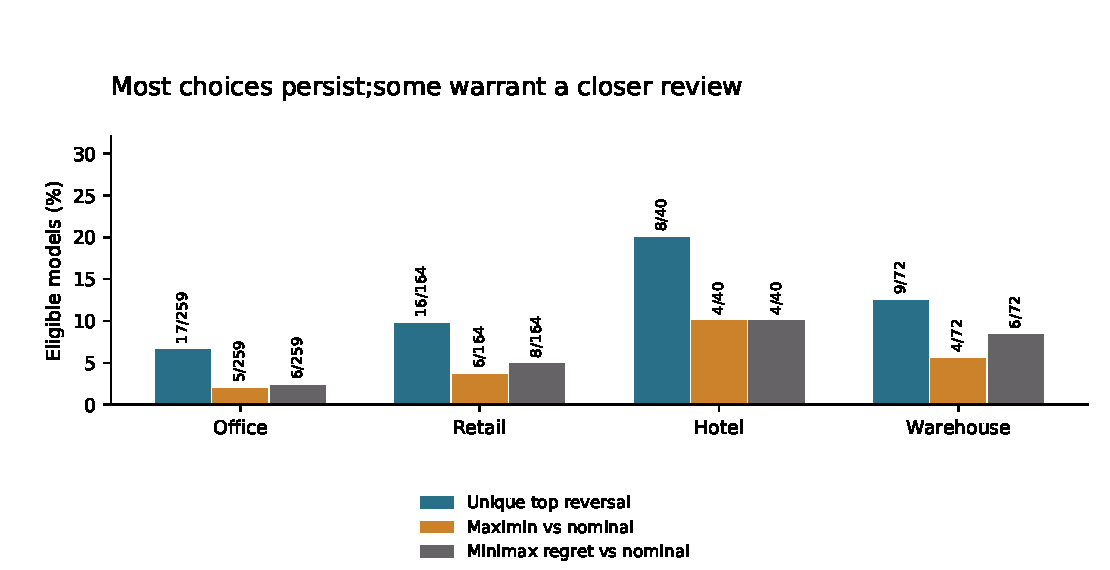
\includegraphics[width=\linewidth]{images/choice_changes.pdf}\end{center}
\captionof{figure}{All eligible groups. Blue compares unique top-ranked alternatives between the published cases; the other bars compare fixed-rule choices with nominal. Labels give exact counts and denominators. A changed choice is a review flag, not proof that a retrofit is worthwhile.}

\textbf{Practical next step.} Inspect the alternative, scenario gains and regret for each changed model ID. Obtain actual building characteristics, installed cost, tariffs and field validation before making an investment decision. These unweighted modeled cases establish neither realized savings nor a recommendation for a particular physical building.
\newpage
\section*{1. Source and population: model IDs, not physical buildings}
ComStock supplies physics-based building-stock simulation results. Its reference documentation and source attribution are given in [1--3]. This analysis uses \textbf{2025 Release 2}, AMY2012 and AMY2018, for Chittenden County, Vermont (GISJOIN G5000070). It captures baseline 0 and separate upgrades 39 LED Lighting, 40 Lighting Controls, 45 Roof Insulation and 48 New Windows. No new EnergyPlus simulation is run.

The precollection protocol was committed at \texttt{557cb7c}. Ten exact public Parquet responses were saved once with UTC start/end, status, headers, bytes and SHA-256 before parsing. The selected factual projection has 28,510 source rows. PyArrow and an independent DuckDB decoder reconcile every selected native state and value in 342,144 comparisons. Annual energy is in kWh, area in square feet and reported operating duration in hours. Numeric ratios use exact fractions of retained decimal representations, not physically exact energy measurements.

Source model reuse can produce repeated geographic allocation records. There are 8,700 model/weather/upgrade key groups and 19,810 repeated source rows. All repeated selected technical projections agree literally in this capture; each full model ID counts once. Weighting those copies as independent buildings would inflate the sample. Source weights and national stock totals are not used.

\begin{center}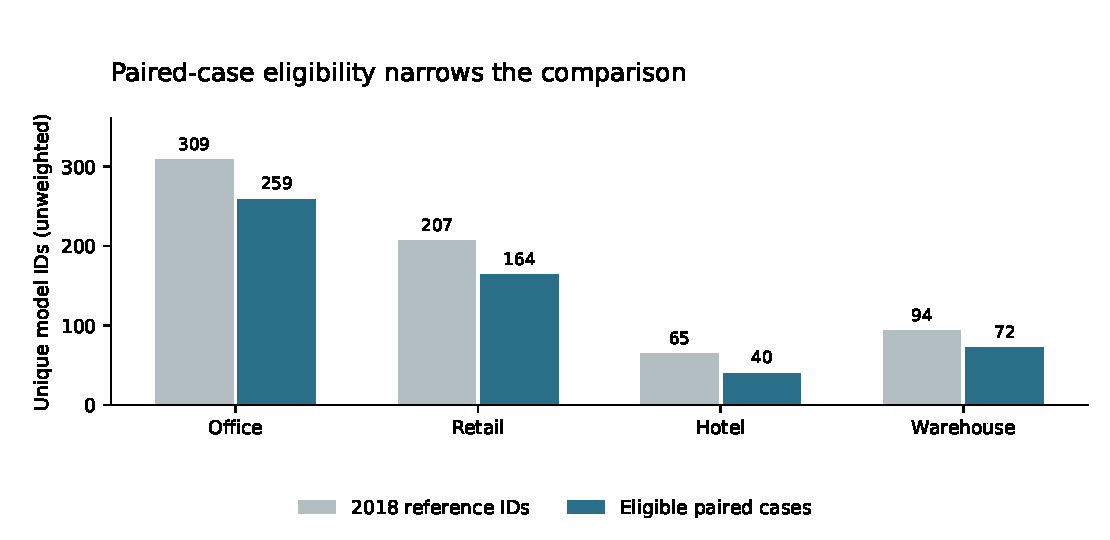
\includegraphics[width=.9\linewidth]{images/cohort_coverage.pdf}\end{center}
\captionof{figure}{Coverage for the four planned analysis groups. All exclusions and source copies remain in machine-readable ledgers. Counts are unique unweighted simulation IDs.}
\begin{center}\begin{tabular}{lrr}\toprule Group & 2018 reference IDs & Eligible paired IDs\\\midrule
Office & 309 & 259 \\
Retail & 207 & 164 \\
Hotel & 65 & 40 \\
Warehouse & 94 & 72 \\
\bottomrule\end{tabular}\end{center}
Across all source types, the 2018 reference population has 882 IDs and 535 qualify for analysis. Another 219 reference IDs lack the 2012 baseline and upgrade records, including IDs outside the four groups; exclusion reasons overlap. Missing scenarios are unknown, never zero gain. The entire source ledger also retains 2012-only IDs outside the reference population.
\newpage
\section*{2. Fixed feasible sets and decision rules}
For eligible model $i$, action $a$ and supplied case $w$, site-energy gain is
\[
 g_i(a,w)=100\frac{E_i(0,w)-E_i(a,w)}{E_i(0,w)}.
\]
Units are percentage points of that case's baseline site energy. No action has gain zero. Negative gains remain negative. Electricity differences and their own baseline-normalized quantities are exported separately; neither is a tariff, carbon factor or monetary return. Separate measure results are never added into an unmodeled package, following the publisher's warning [4].

Both baseline cases require source Success, finite positive site energy and area, and finite nonnegative electricity and reported durations. Type, area and durations must agree between baseline cases. Every proposed alternative needs a source record in both cases. Explicit false applicability in both removes the action; true in both requires Success and finite nonnegative energy. Missing, conflicting, failed or unknown inputs trigger full-model abstention rather than a favorable incomplete comparison. Baseline-only cases remain outside the multi-action denominator.

\begin{center}\begin{tabular}{lp{4.7in}}\toprule Rule & Objective over the same feasible actions\\\midrule
Nominal & Maximize $g_i(a,2018)$.\\
Maximin & Maximize $\min_w g_i(a,w)$.\\
Minimax regret & Minimize $\max_w[\max_b g_i(b,w)-g_i(a,w)]$.\\\bottomrule\end{tabular}\end{center}
Exact objective ties prefer the lower numeric upgrade ID, with no action first. Full tied-top sets, case ranks and Pareto dominance are exported for every alternative. A strict reversal requires a unique top in each case and different actions; a change involving a tie is reported separately. Equal-case averages describe these two cases and do not assign future-weather probabilities.

\textbf{What is mathematical, and what is observed.} Maximin cannot have a worse within-set minimum gain than nominal. Minimax regret cannot have a worse within-set maximum regret. These properties are implementation checks, not empirical discoveries. The observed contributions are the count and identity of changed choices, their magnitudes, applicability and adverse outputs in this specific source cohort. Neither criterion establishes cost effectiveness or robustness outside the assumed cases.

\textbf{Separation before held summaries.} Office and Retail are development archetypes. Hotel and Warehouse are held descriptive archetypes. No parameters are learned and no rule is selected on development performance. Twenty-eight dependency hashes, including the protocol, source, qualification, rule/checking code, fixtures and development outputs, were committed at \texttt{c61da1c} before held decision summaries. Full IDs cannot cross roles. This is not a random-sample or unknown-weather forecast test: both source cases are known optimization inputs.

\textbf{Duration diagnostics.} Fixed weekday bands are at most 8 hours, above 8 through 12 hours, and above 12 hours. The thresholds are declared diagnostics, not calibrated operating cutoffs. These are source-reported modeled durations, not measured occupancy counts or a controlled occupancy perturbation. The selected baseline inputs match, but the two published cases may differ in calendar or other execution details. They do not isolate a causal weather effect.
\newpage
\section*{3. Development: retain the small differences and the adverse cell}
Development contains 423 unique Office and Retail IDs. All three fixed rules are retained. The table reports means over IDs, without stock weights; worst gain and worst regret are first computed per ID across the two source cases, then averaged. Gain and regret columns are percentage points, not percentages of currency or realized energy savings.
\begin{center}\small\begin{tabular}{lrrrrrr}\toprule
Rule & IDs & 2018 gain & 2012 gain & Worst gain & Worst regret & Changed\\\midrule
Nominal & 423 & 6.272 & 6.286 & 6.015 & 0.049 & 0 \\
Maximin & 423 & 6.266 & 6.316 & 6.025 & 0.025 & 11 \\
Minimax regret & 423 & 6.262 & 6.324 & 6.022 & 0.022 & 14 \\
\bottomrule\end{tabular}\end{center}
There are 33 strict unique-top reversals and 34 top-set changes. The difference is a change involving a tie, retained in the diagnostic export. One should not describe every top-set change as a strict ranking reversal. 1 applicable action/case cell has negative site-energy gain; it remains in the outputs and no-action alternative set.

\begin{center}\small\begin{tabular}{lrrrrr}\toprule
Group / duration & IDs & Strict flips & MM changed & Nominal regret & MM regret\\\midrule
Office & 259 & 17 & 6 & 0.049 & 0.023 \\
Retail & 164 & 16 & 8 & 0.049 & 0.019 \\
(8,12]hr & 216 & 17 & 9 & 0.062 & 0.023 \\
$\leq$8hr & 140 & 12 & 3 & 0.038 & 0.027 \\
$>$12hr & 67 & 4 & 2 & 0.032 & 0.006 \\
\bottomrule\end{tabular}\end{center}
MM denotes minimax regret; regret columns are mean worst-case percentage points. Group and duration rows are separate diagnostics and overlap; they must not be added together. Complete source-building-type results are also exported. The fixed band definitions do not create independent replications or a claim that a specific duration causes a different retrofit effect.

The development comparison was used to check implementation and reporting. Independent exact-rational objective enumeration verifies 87,283 fields or structural conditions, including every feasible alternative, tie, dominance state, rule choice and group metric. Twenty-nine finite fixtures cover negative gains, no action, close exact values, complete ties, objective differences, copy conflicts, null/false distinctions and role disjointness. These finite checks do not establish universal correctness or source-model accuracy.

An early development export exceeded Python's default integer-to-string limit because exact aggregate rational denominators can be long. The failed code and failure evidence are preserved. The repair changes bounded local serialization, not comparisons, tolerances, measures or results. No held summary existed then. A later figure consumer required the same reader setting; its partial artifacts are also retained. The current exports and figures pass fresh checks.
\newpage
\section*{4. Held archetypes: limited changes, finite-scenario tradeoffs}
The frozen rules are applied to 112 Hotel and Warehouse IDs. This application changes the archetype composition; it does not withhold the weather cases from the optimization. No held result is used to change an action, objective, tie convention, cohort gate or stratum.
\begin{center}\small\begin{tabular}{lrrrrrr}\toprule
Rule & IDs & 2018 gain & 2012 gain & Worst gain & Worst regret & Changed\\\midrule
Nominal & 112 & 6.639 & 6.579 & 6.285 & 0.119 & 0 \\
Maximin & 112 & 6.625 & 6.653 & 6.299 & 0.059 & 8 \\
Minimax regret & 112 & 6.614 & 6.670 & 6.296 & 0.053 & 10 \\
\bottomrule\end{tabular}\end{center}
\begin{center}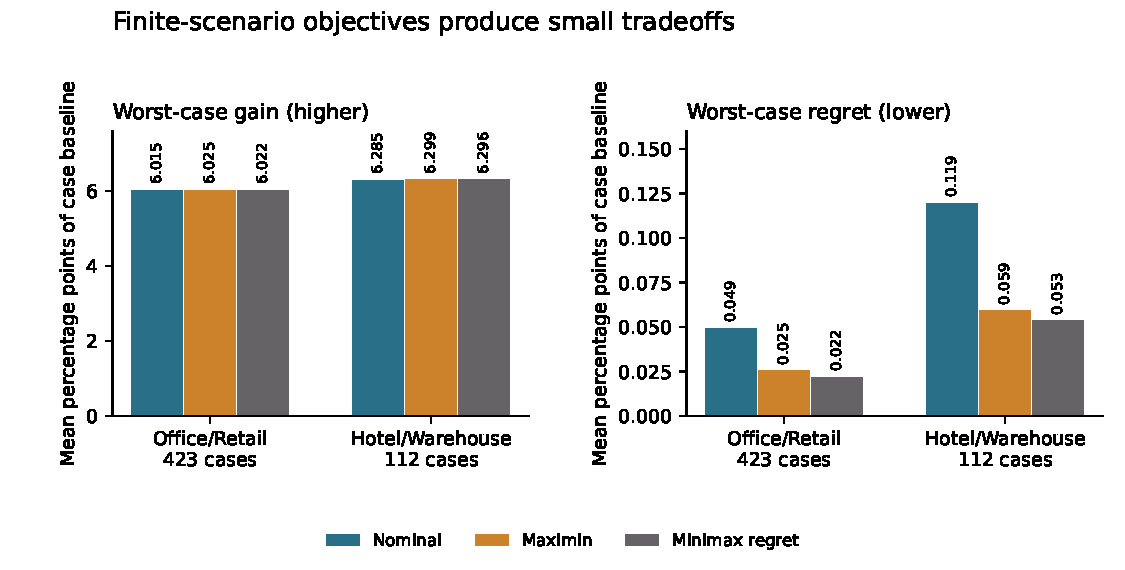
\includegraphics[width=\linewidth]{images/scenario_tradeoffs.pdf}\end{center}
\captionof{figure}{Per-ID worst-case gains and regrets, averaged over each role. Each panel starts at zero and has its own scale. Small differences are visible in labels. Objective inequalities follow from the finite optimization, not field validation.}
\begin{center}\small\begin{tabular}{lrrrrr}\toprule
Group / duration & IDs & Strict flips & MM changed & Nominal regret & MM regret\\\midrule
Hotel & 40 & 8 & 4 & 0.082 & 0.060 \\
Warehouse & 72 & 9 & 6 & 0.140 & 0.050 \\
(8,12]hr & 44 & 11 & 6 & 0.234 & 0.111 \\
$\leq$8hr & 31 & 2 & 1 & 0.041 & 0.028 \\
$>$12hr & 37 & 4 & 3 & 0.049 & 0.006 \\
\bottomrule\end{tabular}\end{center}
There are no held changes involving a tie and no held applicable action/case cell with negative site-energy gain. That finite observation does not rule out adverse results elsewhere. Maximin and minimax regret make different compromises: their objectives are not interchangeable. Independent enumeration checks 23,087 held fields or structural conditions. Do not promote a mathematically preferred score into a claim that a retrofit should be purchased.
\newpage
\section*{5. Reproduction, limitations and an implementation exercise}
\textbf{Reproduce the decision trail.} The repository retains the complete selected source projection, dictionary bindings, source manifest, copy and exclusion ledgers, exact scenario inputs, all alternatives, rule choices, ties and cohort/stratum summaries. Independent SQL/Decimal qualification checks 328,115 conditions before scoring. Original Parquet files remain privately retained and were independently decoded; public hash/schema checks do not repeat private-original decoding.

Run \texttt{python src/reproduce.py} from a full-history checkout. It clones the committed study locally, regenerates into a separate temporary directory, and compares 447,801 CSV fields including headers and six JSON documents. It runs independent checks, 29 fixtures and the committed freeze proof while preserving original files. Local replay passes with Python 3.10 and 3.12.14. It performs no source-network access and preserves frozen compression containers. A separate figure checker recomputes 32 plotted values from individual ledgers, verifies 256 actual SVG coordinates and nine artifact hashes. A manuscript checker independently reconstructs all ledgered numerical displays and verifies the five scoped paper files. These are bounded artifact checks, not physical validation.

\textbf{Implementation exercise.} Choose a changed model from \texttt{held\_choices.csv}; join its full alternative outcomes and exclusion/feasibility records. Recompute the three rules from the two exact source-case gains. Explain whether the change comes from worst gain, regret or a tie. Then list the missing inputs needed for a real decision: site verification, actual costs, tariffs, intervention feasibility and a defensible scenario set. Do not introduce an invented cost or turn a missing scenario into zero. The separate paper-recommendation product in the research program covers recommendation-engine implementation; this exercise covers transparent finite decisions.

\textbf{Limits.} One county, two published simulation cases and a selected set of four measures cannot establish national effects or future-weather reliability. Source model reuse is resolved only for the selected projection; matching those inputs is not a complete independent audit of every EnergyPlus configuration. Duration groups are not occupancy experiments. The source calendar and execution details may confound a weather-only interpretation. No causal effect, installed cost, actual energy saving, customer adoption, deployment, statistical significance, new estimator or scientific priority is claimed. This is an independent program manuscript, not peer reviewed. Formal-publication projects, including Azure optimization, remain private.

\textbf{Data attribution and changes.} The factual subset comes from ComStock, developed by the National Laboratory of the Rockies with U.S. Department of Energy funding. The source collection links CC BY 4.0; source URLs, attribution and change notices are retained. This analysis selects fields, collapses identical technical copies and computes new ratios and decisions. The publisher provides data for research as-is, with no duty to maintain or confirm accuracy. No endorsement is implied. Known mislabeled packages 55/58 and Hawaii weather issues are outside this fixed cohort [5].

\small
[1] Parker, A., et al. (2023). \emph{ComStock Reference Documentation}. NREL/TP-5500-83819. \url{https://www.nlr.gov/docs/fy23osti/83819.pdf}.

[2] ComStock dataset catalog. 2025 Release 2, AMY2012 and AMY2018. \url{https://comstock.nlr.gov/page/datasets}. Exact file URLs and capture hashes are in the source manifest.

[3] OEDI, \emph{End-Use Load Profiles for the U.S. Building Stock}, DOI 10.25984/1876417. \url{https://data.openei.org/submissions/4520}. Attribution/disclaimer: \url{https://natlabrockies.github.io/ComStock.github.io/docs/citation.html}.

[4] ComStock, \emph{Why Individual ComStock Measure Results Should Not Be Combined}. \url{https://natlabrockies.github.io/ComStock.github.io/docs/resources/explanations/combining_measure_results.html}.

[5] ComStock, \emph{2025 Release 2 Packages Known Issue}. \url{https://natlabrockies.github.io/ComStock.github.io/docs/resources/explanations/2025_release_2_packages_known_issue.html}. Source pages checked 30 October 2026.
\end{document}
